\documentclass[11pt]{article}
\renewcommand{\baselinestretch}{1.05}
\usepackage{amsmath,amsthm,verbatim,amssymb,amsfonts,amscd, graphicx}
\usepackage{graphics}
\usepackage{tikz}
\usepackage{pgfplots}
\topmargin0.0cm
\headheight0.0cm
\headsep0.0cm
\oddsidemargin0.0cm
\textheight23.0cm
\textwidth16.5cm
\footskip1.0cm
\parindent0pt
\theoremstyle{plain}
\newtheorem{theorem}{Theorem}
\newtheorem{corollary}{Corollary}
\newtheorem{lemma}{Lemma}
\newtheorem{proposition}{Proposition}
\newtheorem*{surfacecor}{Corollary 1}
\newtheorem{conjecture}{Conjecture}
\newtheorem{question}{Question}
\theoremstyle{definition}
\newtheorem{definition}{Definition}
\let\mbb\boldsymbol
\renewcommand\boldsymbol{\mbb}
\renewcommand{\a}{\"{a}}
\renewcommand{\o}{\"{o}}
\renewcommand{\u}{\"{u}}
\newcommand{\beequal}{\mathop{=}\limits^!}

\begin{document}

\title{Numerische Mathematik f\u r Ingenieure (SS 14) - \"{U}bung 5}
\author{Merikan Koyun \& Julian Andrej}
\maketitle

\section*{T8.) Beispiel einer nichtlinearen Gleichung}
Mit Hilfe des Banach'schen Fixpunktsatzes soll gezeigt werden, dass es genau ein $x \in [0,\pi]$ gibt, welches 
\begin{equation}
\frac{1}{5}\sin(x)\cos(x) = \frac{2x-3}{6}
\label{eq}
\end{equation}
l\o st.\\
Falls $\Phi$ einen Fixpunkt besitzt, gilt $\Phi(x) = x$. Umgeformt ergibt sich also f\u r die Gleichung:
\begin{align}
\Phi(x) = \frac{3}{5}\sin(x)\cos(x)+\frac{3}{2}
\end{align}

Laut Fixpunktsatz von Banach gilt f\u r eine Iteration $\Phi$ auf einer abgeschlossenen Menge $U \subseteq R^n$ und $x,y \in U$:
\begin{equation}
\Vert \Phi(x)-\Phi(y) \Vert \leq L \Vert x-y \Vert \qquad \text{mit } L \in [0,1)
\end{equation}
Ist dies erf\u llt, dann besitzt $\Phi$ genau einen Fixpunkt und die Fixpunktiteration iteriert f\u r beliebige Startwerte $x \in U$.

Um $L$ zu bestimmen benutzen wir den Mittelwertsatz der Differentialrechnung:
\begin{equation}
\Phi(x)-\Phi(y) \leq \Phi'(\eta) (x-y)
\end{equation}

Mit diesem Ansatz ergibt sich:
\begin{equation}
|\Phi(x)- \Phi(y) | = |\Phi'(\eta)||x-y| \qquad \text{mit } x,y \in [0,\pi]
\end{equation}
mit $\eta \in [0,\pi]$ von $x$ und $y$ abh\a ngige Zwischenpunkte.
Es gilt:
\begin{equation}
|\Phi'(\eta)| = \left|\frac{3}{5}\cos(2 \eta)\right| \leq 0.6 \quad \forall \eta
\end{equation}
Nun muss noch gepr\u ft werden, ob $\Phi$ das Intervall $[0, \pi]$ auf sich selbst abbildet. Es gilt:
\begin{equation}
\Phi(0)=\frac{6}{5} \geq 0 \qquad \Phi(\pi) = \frac{9}{5} \leq \pi
\end{equation}
$\Phi$ bildet das Intervall $[0, \pi]$ auf sich selbst ab.
Somit l\a sst sich $L=0.6 \in [0,1)$ setzen. Demnach ist $\Phi$ eine Kontraktion und die Gleichung \eqref{eq} besitzt genau einen Fixpunkt.

\section*{T9.) Newton-Verfahren an einem Beispiel}
Gegeben ist die Funktion $f(x)=x^3 - 3x^2 + x -3$. Die Ableitung lautet $f'(x)=3x^2 - 6x+1$. Die Iterationsvorschrift des Newton-Verfahrens ist wie folgt definiert:
\begin{equation}
x \rightarrow x - \dfrac{f(x)}{f'(x)} = x - \dfrac{x^3 - 3x^2 + x -3}{3x^2 - 6x+1}
\end{equation}

% X = 0 %%%%%%%%%%%%%%%%%%%%%%%%%%%%%%%%%%%%%%%%%%%%%%%%%%%%%%%%%%%%%%%%%%%%%%
%%%%%%%%%%%%%%%%%%%%%%%%%%%%%%%%%%%%%%%%%%%%%%%%%%%%%%%%%%%%%%%%%%%%%%%%%%%%%%
Bei $x_0=0$ ergeben sich also folgende Iterationsschritte:
\begin{align*}
x_0 = 0, \quad x_1 = 3, \quad x_2 = 3 
\end{align*}

\begin{figure}[!ht]
\centering
\begin{tikzpicture}
    \begin{axis}[
    axis lines=middle,
    axis line style={-latex},
    x label style={at={(axis description cs:0.5,-0.1)},anchor=north},
    y label style={rotate=90,anchor=north}]
	\addplot[black,samples=100,domain=-2:3.9] {x^3 - 3*x^2 + x - 3};
	\addplot [green, mark=*, mark options={draw=black}, only marks]
	coordinates {
	(0,-3) 
	};	
	\addplot [red, mark=*, mark options={draw=black}]
	coordinates {
	(3,0)	
	};
	\node at (axis cs:0,-3) [anchor=north west] {$x_0$};
	\node at (axis cs:3,0) [anchor=south east] {$x_1,\,x_2$};
	\node at (axis cs:3.8,0) [anchor=north east] {$x$};
	\node at (axis cs:0,11) [anchor=south west] {$f(x)$};
	\end{axis}
\end{tikzpicture}

\title{Visualisierung f\u r $x_0=0$}
\end{figure}

Es l\a sst sich erkennen, dass das Newton-Verfahren in einem Schritt zu der Nullstelle konvergiert. Die schnelle Konvergenz ausgehend von diesem Startpunkts l\a sst sich anhand der Tangente in diesem Punkt begr\u nden. Diese geht direkt durch den Punkt $(3,0)$, der offensichtlich eine Nullstelle ist und somit konvergiert das Verfahren in einem Schritt.\vspace{0.3cm}

% X = 0.5 %%%%%%%%%%%%%%%%%%%%%%%%%%%%%%%%%%%%%%%%%%%%%%%%%%%%%%%%%%%%%%%%%%%%
%%%%%%%%%%%%%%%%%%%%%%%%%%%%%%%%%%%%%%%%%%%%%%%%%%%%%%%%%%%%%%%%%%%%%%%%%%%%%%
Bei $x_0=0.5$ ergeben sich folgende Iterationsschritte:
\begin{align*}
x_0 = 0.5, \quad x_1 = -2, \quad x_2 = -1 
\end{align*}

\begin{figure}[!ht]
\centering
\begin{tikzpicture}
    \begin{axis}[
    axis lines=middle,
    axis line style={-latex},
    x label style={at={(axis description cs:0.5,-0.1)},anchor=north},
    y label style={rotate=90,anchor=north}]
	\addplot[black,samples=100,domain=-2:3.9] {x^3 - 3*x^2 + x - 3};
	\addplot [green, mark=*, mark options={draw=black}, only marks]
	coordinates {
	(0.5,-3.125) 
	};	
	\addplot [red, mark=*, mark options={draw=black}, only marks]
	coordinates {
	(-2,-25)
	(-1,-8)	
	};
	\node at (axis cs:0,-3) [anchor=north west] {$x_0$};
	\node at (axis cs:-1.9,-25) [anchor=south west] {$x_1$};
	\node at (axis cs:-1,-8) [anchor=south east] {$x_2$};
	\node at (axis cs:3.8,0) [anchor=north east] {$x$};
	\node at (axis cs:0,11) [anchor=south west] {$f(x)$};
	\end{axis}
\end{tikzpicture}

\title{Visualisierung f\u r $x_0=0.5$}
\end{figure}

Hier l\a sst sich erkennen, dass sich das Newton-Verfahren von der gesuchten Nullstelle entfernt, da die Tangente am Startpunkt eine negative Steigung aufweist, und sich somit der neue Iterationsschritt in negative $x$-Richtung bewegt. Nach diesem Schritt zeigt die Tangente nun wieder in Richtung der Nullstelle, \a hnlich wie bei $x_0=0$. Das Verfahren n\a hert sich also wieder der Nullstelle und wird schlussendlich auch wieder zur Nullstelle konvergieren, jedoch mit einer wesentlich h\o heren Anzahl an Iterationsschritten als im Fall zuvor.\vspace{0.3cm}


% X = 0.4 %%%%%%%%%%%%%%%%%%%%%%%%%%%%%%%%%%%%%%%%%%%%%%%%%%%%%%%%%%%%%%%%%%%%
%%%%%%%%%%%%%%%%%%%%%%%%%%%%%%%%%%%%%%%%%%%%%%%%%%%%%%%%%%%%%%%%%%%%%%%%%%%%%%
Bei $x_0=4$ ergeben sich folgende Iterationsschritte:
\begin{align*}
x_0 = 4, \quad x_1 = 3.32, \quad x_2 = 3.05 
\end{align*}

\begin{figure}[!ht]
\centering
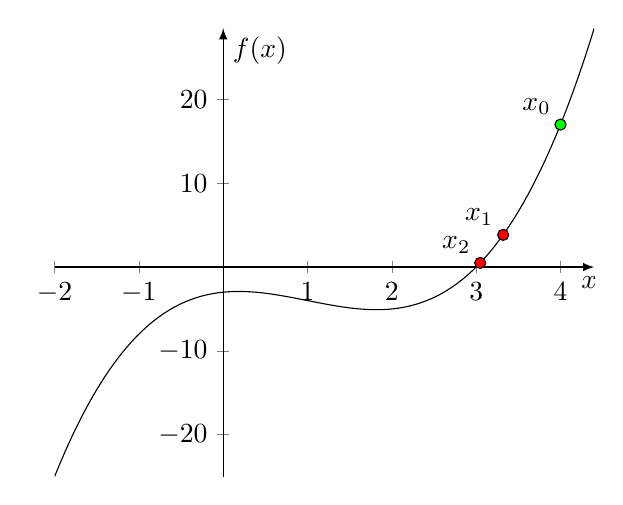
\begin{tikzpicture}
    \begin{axis}[
    axis lines=middle,
    axis line style={-latex},
    x label style={at={(axis description cs:0.5,-0.1)},anchor=north},
    y label style={rotate=90,anchor=north}]
	\addplot[black,samples=100,domain=-2:4.4] {x^3 - 3*x^2 + x - 3};
	\addplot [green, mark=*, mark options={draw=black}, only marks]
	coordinates {
	(4,17) 
	};	
	\addplot [red, mark=*, mark options={draw=black}, only marks]
	coordinates {
	(3.32,3.84) 
	(3.0481, 0.4950)	
	};
	\node at (axis cs:4,17) [anchor=south east] {$x_0$};
	\node at (axis cs:3.32,3.84) [anchor=south east] {$x_1$};
	\node at (axis cs:3.0481, 0.4950) [anchor=south east] {$x_2$};
	\node at (axis cs:4.55,0) [anchor=north east] {$x$};
	\node at (axis cs:0,23) [anchor=south west] {$f(x)$};
	\end{axis}
\end{tikzpicture}

\title{Visualisierung f\u r $x_0=4$}
\end{figure}
Das Newton-Verfahren konvergiert fast vollst\a ndig in zwei Schritten (quadratische Konvergenz) zur Nullstelle.

\end{document}
